\documentclass[a4paper,12pt]{article}

\usepackage{url}
\usepackage{epsfig}
\usepackage{graphics}
\usepackage{fancyhdr}

\graphicspath{{pictures/}}

\title{Report template for the project in the course DD2380 at KTH}
\author{\hspace*{-0.5cm}
GROUP31\\
\begin{tabular}{cc}
Akash Patel & Christoph Kaiser \\
 921119-3256	 & 920416-T336\\
19/11/92 & 16/04/92 \\
akash@kth.se & ckai@kth.se \\
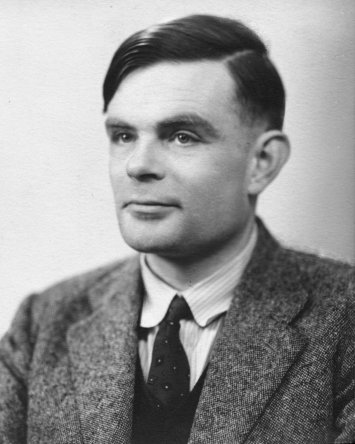
\includegraphics[width=0.13\linewidth]{Alan_Turing_photo} & 
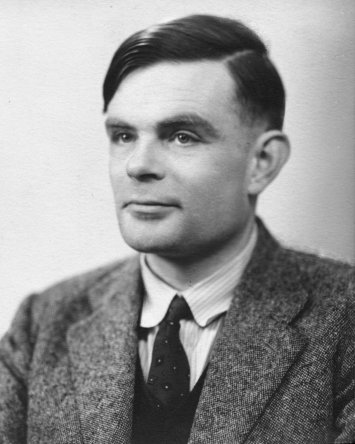
\includegraphics[width=0.13\linewidth]{Alan_Turing_photo} \\
& \\
 Lisa Schmitz & Nikolaos Tatarakis\\
 920606-T203		&\\
 06/06/92 & BIRTHDATE4 \\
 lschmitz@kth.se & MAIL4@kth.se \\

\includegraphics[width=0.13\linewidth]{lisaSchmitz_photo} &
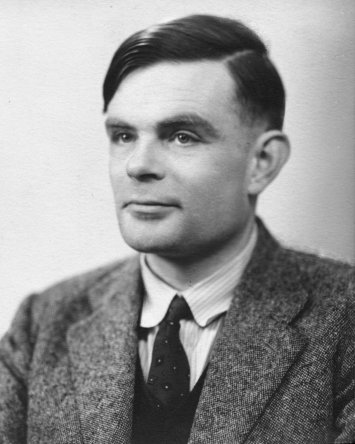
\includegraphics[width=0.13\linewidth]{Alan_Turing_photo}
\end{tabular}} 
% Normally there will not be any pictures but we want
% these so that we can connect faces to names in the course
% We also want birthdates so that we can tell people with the same
% name apart
\date{}

\pagestyle{fancy}
\setlength{\headheight}{15pt}
\fancyhf{}
\lhead{DD2380 ai15} % DO NOT REMOVE!!!!
\rhead{A. Patel, C. Kaiser, L. Schmitz, N. Tatarakis} %% UPDATE WITH YOUR NAMES
\fancyfoot[LE,RO]{\thepage}
\begin{document}

\maketitle
\thispagestyle{fancy}

\begin{abstract}

\end{abstract}
This paper explores the potential accuary of the analysis of song lyrics. Different text analysers were tested for their ability to categorize lyrics as \textit{negative} or \textit{positive}. The focus lies on the comparison of different feature extraction methods and classifier. The identification of emotion in lyrics is a problem which has no satisfying solution yet.

\clearpage

%%%%%%%%%%%%%%%%%%%%%%%%%%%%%%%%%%%%%%%%%%%%%%%%%%%%%%%%%%%%%
%%%%%%%%%%%%%%%%%%%%%%%%%%%%%%%%%%%%%%%%%%%%%%%%%%%%%%%%%%%%%
\section*{NOTE}
Related Works, Experimental Results, Discussions, Summary are sections that MUST be contained.

 The section \textit{Contributions} is a place to express any difference in contributions. The default assumption is that you all agree that all of you had an equal part to play in the project.

\section{Introduction (1--2 pages)}
\label{sec:intro}

Music has a great impact on people. Everyone knows the phenomen that a song can influence our mood, it can make us sad and it can make us happy. This amazing control over people's feelings is something which can be used for many different purposes. For example music provider like Spotify offer playlists labelled with a certain mood. But industries are not the only area of application. Researchers see a use for it in edutainment and even psychological therapy\,\cite{kim2010music}. Unfortunately, the task of predicting the correct assoziated mood is not an easy one due to the comlexity of how emotion is transferred in songs. Obviously emotion is encoded both in the audio and the lyrics of a song\,\cite{yang2008regression}. This paper compares methods to identify emotion by analysing the text of song lyrics. In order to do this different variants of text analysers were tested. The modification was conducted by using different categories of emotions and classifiers. 

\subsection{Contribution}


\subsection{Outline}
Since our work deals with different approaches of categorising and classifying song lyrics, previous work should be taken into count. The related work is therefore presented in Section~\ref{sec:relwork}. We based our text analyser in the results of this previous studies. Section~\ref{sec:method} explains the method we used to realise and implement the analyser in detail. We used different variations of our text analyser, modifying the the categorsiation and the classifier. The results we were able to gather are described in  Section~\ref{sec:exps}. Moreover, problems that came up during the research are mentioned in this section. The results are sumarized in  Section~\ref{sec:summary} and possible further research areas are given eventually.

%%%%%%%%%%%%%%%%%%%%%%%%%%%%%%%%%%%%%%%%%%%%%%%%%%%%%%%%%%%%%
%%%%%%%%%%%%%%%%%%%%%%%%%%%%%%%%%%%%%%%%%%%%%%%%%%%%%%%%%%%%%
\section{Related work}
\label{sec:relwork}
Our work is mainly based the on paper of Youngmoo E. Kim et al.\,\cite{kim2010music}. It gives an overview of recent approaches of emotion recognition in lyrics.  Most of the presented approaches are content-based and are therefore relevant references for our work. Not only do they deal with different categorisations of mood but also treat variations of classifiers. This work provides a good inside into what has already been done and what worked well. Therefore it can be seen as the foundation we built our work on. We realised some of the presented methods and compared them to each other. 

Different bag-of-words model classifiers are explained by Li et al.\,\cite{li1998classification}.

%%%%%%%%%%%%%%%%%%%%%%%%%%%%%%%%%%%%%%%%%%%%%%%%%%%%%%%%%%%%%
%%%%%%%%%%%%%%%%%%%%%%%%%%%%%%%%%%%%%%%%%%%%%%%%%%%%%%%%%%%%%
\section{Method}
\label{sec:method}

Bla bla bla bla bla bla bla bla bla bla bla bla bla bla bla bla bla 
bla bla bla bla bla bla bla bla bla bla bla bla bla bla bla bla bla 
bla bla bla bla bla bla bla bla bla bla bla bla bla bla bla bla bla 

\subsection{Implementation}
\label{sec:impl}

The basic model we used for our text analyser is the bag-of-words model\,\cite{Mitchell}. The functionality is illustrated in the figure \ref{fig:bagOfWords}. In this model a database with labeled data such as lyrics are stored. The next step would be to preprocess the lyrics and create a dicitonary with $n$-grams based on it. The database is divded into two parts: a training and a test set. Using this data, a classifier is trained with a training set and its accuracy can then be evaluated with the classification of the test set. In the following abstracts the individual parts of the bag-of-words model will be explained in detail. 

\begin{figure}
\centering
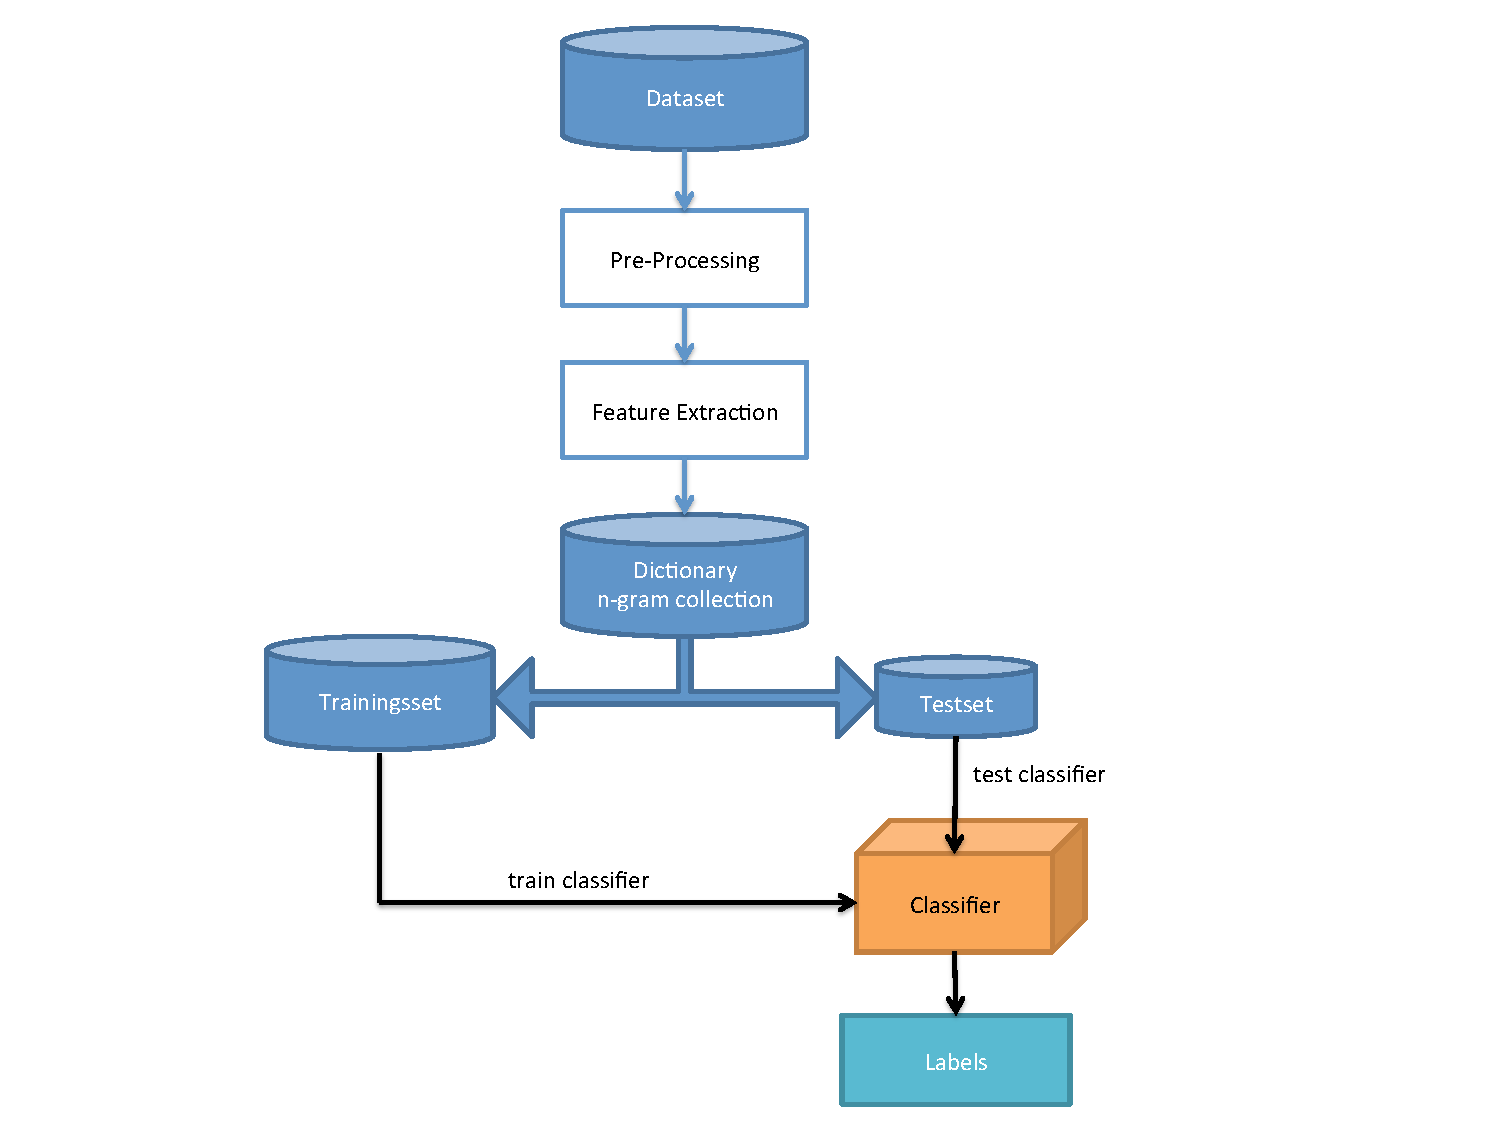
\includegraphics[width=0.8\linewidth]{flowChartBagOfWords}
\caption{A description that makes browsing the paper easy and clearly 
describes what is in the picture. Make sure that the text in the figure 
is large enough to read and that the axes are labelled.}
\label{fig:bagOfWords}
\end{figure}

\paragraph{Database} The database was one of the most difficult parts of this research. Due to copyright issues it was not possible to access a already available database and we had to built one on our own. Some earlier researches use \texttt{Allmusic.com} as a basis for the database \cite{kim2010music}, since it provides emotional labels for songs. For this reason a program has been written to extract the lyrics with its song's emotional label. 

Even though this prelabeling of the songs was helpful, with over ... emotional labels it were simply to many categories to use. Therefore we had to find supercategories for the existing labels. Downie et al. suggest in \,\cite{downie20082007}  to use five clusters of emotions. Whereas Yang and Lee only suggests a binary distinction into positive and negative emotions\,\cite{yang2009music}. Both variants were tested during our research.

\paragraph{Pre-processing} The lyrics have been pre-processed the same way for each of the variants of the text analyser. Stop-words are filtered out using the Natural Language Toolkit and special character are deleted. In a next step, every word of the lyric is stemmed which means that it is transferred into its basic form. For example "wait" and "waiting" would be interpreted as the same word after the stemming has been done. The pre-processing is performed due to avoid misclassifications. 

\paragraph{Feature extraction} The feature extraction is condtucted for all lyrics. The procedure consists of transferring the lyrics into $n$-gram representation. We considered only 1-, 2- and 3-grams as reasonable parameters which is why only these have been tested in our study. 

\paragraph{Classification} The Natural Language Toolkit and the SciKit-Learn library provide the most commonly used text classifiers. In the following section the tested classifiers will be introduced. 

\begin{itemize}
\item \textit{Naive Bayes} Let $\mathcal{C} = (c_1,\dots,c_n)$ be the categories and $n$ the number of categories. Given a document $\mathcal{D}$ and its word list $\mathcal{W} = (w_1, \dots, w_m)$ with $m$ being the number of words of a certain document, the Naive Bayes classifier determines the category of a document as follows:

$$
c^*_{NB} = argmax_{c_{j \in \mathcal{C}}} P(c_j) \prod^d_{i = 1} P(w_i | c_j)
$$
with $P(c_j)$ being the \textit{a priori} probability of a class $c_j$ and $P(w_i | c_j)$ being the conditional probability of the word $w_i$ given class $c_j$.

Naive Bayes will only work well for large enough datasets. 

\item \textit{Multinomial Naive Bayes}
Multinomial Naive Bayes extends the Naive Bayes algorithm to handle multinomial distributed data. In text analysis this is particularly useful where events represent the occurrence of a word in a document. 

A feature vector $w = (w_1, \dots, w_n)$ is given where $w_i$ counting the number of times a word $i$ was observed in a particular instance. The likelihood of observing a histogram $\mathbf{w}$ is then given by,

$$
 P(\mathbf{w}| c_j) = \frac{(\sum_{i}{w_i})!}{\prod_{i} w_i!}\prod_{i}p^{w_i}_{ji}
$$

Here $p_{ki}$ is part of a multinomial distribution $p_{k}$ and the probability that a word $i$ is observed.

\item \textit{Bernoulli Naive Bayes}
In contrast to the Multinomial NB the Bernoulli NB uses binary term occurrence rather than term frequencies which allows it to penalize non-occuring terms. Although there may be multiple features, each one is assumed to be a binary valued variable. Thus samples are represented as binary feature vectors. The likelihood of a feature vector given a category is given by,

$$
 P(\mathbf{w}| c_j) =\prod_{i} p^{w_i}_{ji}(1-p_{ji})^{1-w_i}
$$


The model is particularly useful for shorter texts where the lack of certain features can tell you more than solely analyzing occurring features. 

\item \textit{Logistic Regression}
Logistic regression is a linear model for classification where the probabilities describing the possible outcomes of a single event are modeled using a logistic function. This model is then used to classify new input data. 

\item \textit{Support Vector Machine}
If input data are overlap and have similar features, SVMs can be used. They essentially perform non-linear separations by transforming input data to higher dimensions with so called Kernels. This is then combined with a Lagrange constraint to find hyperplanes which separates classes with the largest distance. 


\item \textit{Linear Support Vector Machine}
The main difference with linear SVM compared to kernel SVMs is that the  input data is linearly separable and thus a non-linear kernel to transform data to an higher dimension is not necessary. They are particularly useful for data which have a lot of features and thus easier and faster to separate with a hyperplane.

\item \textit{Stochastic gradient descent}
This classifier combines multiple binary classifiers to separate features in input data. These classifiers are then updated using a version of gradient descent to update the parameters and minimize the error. In contrast to normal gradient descent the stochastic version updates the classification parameters for every training example it encounters with respect to the gradient of the error. Traditionally one has to run through the entire training set before calculating the gradient and updating the parameters. This method allows for a faster learning rate compared to batch gradient descent.

\item \textit{Combination of multiple classifiers} We combined all introduced classifier into one classifier. It basically classifies documents according to how many classifiers resulted into a certain category. The category, to which most of the classification results belong to, gets selected as the resulting category of the song.
\end{itemize}

%%%%%%%%%%%%%%%%%%%%%%%%%%%%%%%%%%%%%%%%%%%%%%%%%%%%%%%%%%%%%
%%%%%%%%%%%%%%%%%%%%%%%%%%%%%%%%%%%%%%%%%%%%%%%%%%%%%%%%%%%%%
\section{Experimental results}
\label{sec:exps}
The goal of our experiment was to compare the performance of different variants of the bag-of-words model classification for emotion in lyrics. 
 

\subsection{Experiemntal setup}
In order to compare the performance of the different classifier variants we changed various parameters. The effect of different amounts of emotional categories have been tested, as well as variations of the $n$ of the $n$-grams, the size of the trainingsset and classifiers.


\subsection{Experiment ...}

\paragraph{Drawbacks} We were aware of the difficulty of the task of designing a sufficient lyrics classifier. Especially in the last years a lot of research has been conducted in this area but there is still a lack of a reliable lyrics analyser. But during our research we were able to gain a better inside into the nature of this difficulty. Feelings and emotions are something very personal, and the perception of the emotion which is transferred by a certain songtext highly depends on the person who is reading the lyrics. It is not unusal that two different people might disagree on the general mood of a lyrical text\,\cite{wilson2005recognizing}. This is why it is of supreme importance to select a representative model of categories.

\paragraph{Variations in categorisation} During our research we came to the conclusion that the use of only two categories - positive and negative - seem to have let to an overgeneralisation of emotions. Even the categories itself which were provided by \texttt{Allmusic.com} could not clearly be mapped to one of these two categories. To illustrate the difficulty we discovered, a research has been done. We used a questionnaire were we asked people to evaluate the categories from \texttt{Allmusic.com} as either negative or postive and to do the same with some randomly picked song lyrics. The results are shown in figure \ref{fig:histogram}. It can be seen that there is a significant discrepancy of opinion across participants. This emphasizes the personal perception of emotion. Due to this, it cannot be expected to gain a higher accuracy by a classifier in emotion categorisation.

A second model of categorisation used in this research has been proposed by Downie et al.\,\cite{downie20082007}. They used five cluster of emotion to categorise lyrics as shown in table \ref{tab:moodClusters}.

\begin{table}
\begin{center}
\begin{tabular}{| l | l |}
\hline
\textbf{Clusters} & \textbf{Mood Adjectives} \\ \hline \hline 
Cluster 1 & passionate, rousing, confident, boisterous, rowdy \\ \hline
Cluster 2 & rollicking, cheerful, fun, sweet, amiable/good natured \\ \hline
Cluster 3 & literate, poignant, wistful, bittersweet, autumnal, brooding \\ \hline
Cluster 4 & humorous, silly, campy, quirky, whimsical, witty, wry \\ \hline
Cluster 5 & aggressive, fiery, tense/anxious, intense, volatile, visceral \\ \hline
\end{tabular}
\caption{Clusters of mood adjectives used in the MIREX Audio Mood Classification task\,\cite{downie20082007}.}
\label{tab:moodClusters}
\end{center}
\end{table}

\paragraph{Variations in n-grams} Another parameter we modified was the assignment of $n$ for the $n$-grams. The effect on the accuracy of the classifiers is illustrated by the figures \ref{fig:nGramsEffectTwoMoods} and \ref{fig:nGramsEffectClusters}.

\paragraph{Variations in the size of the training set} 

\paragraph{Variations in classifiers} We tested the different classifiers described in \ref{sec:impl}. The performance of different classifiers for the two mood variant are shown in \ref{fig:classifiersPerformanceTwoMoods} and for the cluster variant are presented in \ref{fig:classifiersPerformanceCluster}. As it can be seen in the figures, the ... classifier yields the best average results for both categorisation variants. The reason why the linear classifier is working well is that the tested data is highly individual. There is a significant variance between song lyrics and this is why a linear distinction is the best choice for the data in the present case.

 

\begin{figure}
\centering
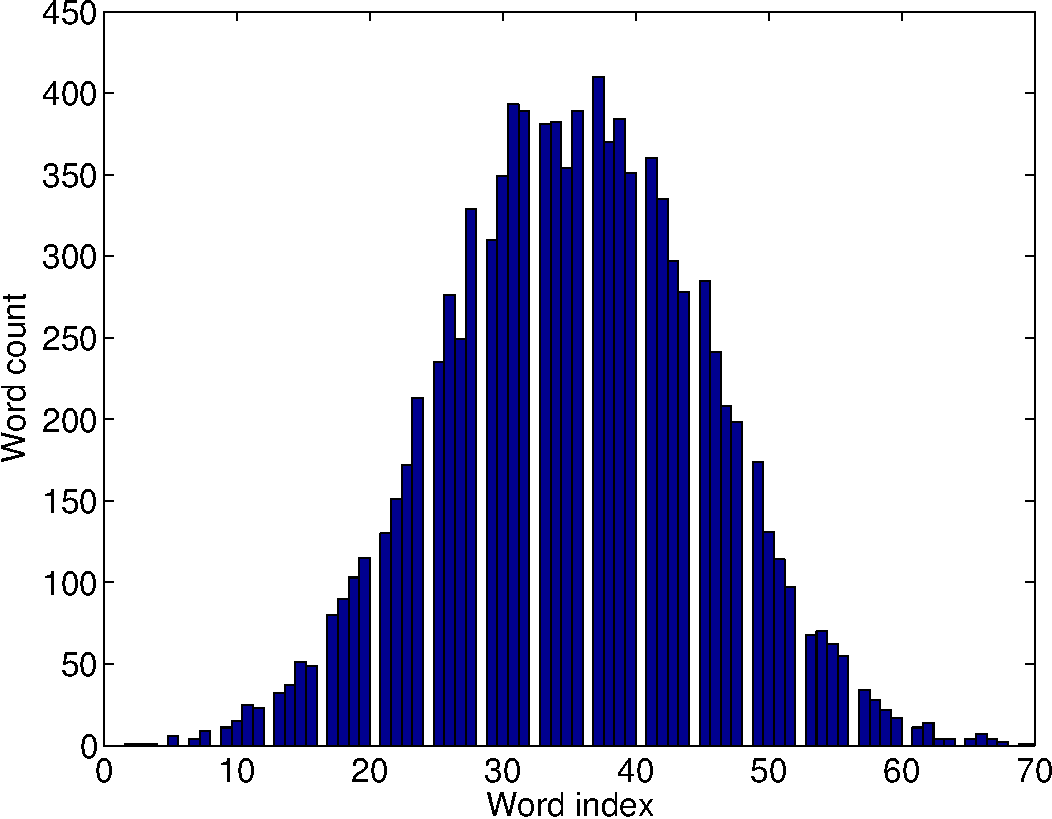
\includegraphics[width=0.8\linewidth]{histogram}
\caption{A description that makes browsing the paper easy and clearly 
describes what is in the picture. Make sure that the text in the figure 
is large enough to read and that the axes are labelled.}
\label{fig:histogram}
\end{figure}
 

%%%%%%%%%%%%%%%%%%%%%%%%%%%%%%%%%%%%%%%%%%%%%%%%%%%%%%%%%%%%%
%%%%%%%%%%%%%%%%%%%%%%%%%%%%%%%%%%%%%%%%%%%%%%%%%%%%%%%%%%%%%
\section{Summary and Conclusions}
\label{sec:summary}

Bla bla bla bla bla bla bla bla bla bla bla bla bla bla bla bla bla 
bla bla bla bla bla bla bla bla bla bla bla bla bla bla bla bla bla 
bla bla bla bla bla bla bla bla bla bla bla bla bla bla bla bla bla 


%%%%%%%%%%%%%%%%%%%%%%%%%%%%%%%%%%%%%%%%%%%%%%%%%%%%%%%%%%%%%
%%%%%%%%%%%%%%%%%%%%%%%%%%%%%%%%%%%%%%%%%%%%%%%%%%%%%%%%%%%%%
\section{Contributions}
\label{sec:contributions}
We the members of project groupXX unanimously declare that 
we have all equally contributed toward the completion of this
project. (PLEASE CHANGE THIS SUITABLY WITH DETAILS, IF IT IS NOT TRUE)


%%%%%%%%%%%%%%%%%%%%%%%%%%%%%%%%%%%%%%%%%%%%%%%%%%%%%%%%%%%%%
%%%%%%%%%%%%%%%%%%%%%%%%%%%%%%%%%%%%%%%%%%%%%%%%%%%%%%%%%%%%%
\bibliographystyle{plain}
\bibliography{reflist}


\end{document}